
\section{Materiais}

%% Tentar fazer a transição deste slide
%\begin{frame}
%\begin{figure}[]
%	\frametitle{Materiais}
%     \centering
%     \captionsetup{width=\textwidth,font=footnotesize,textfont=bf}   
%     \begin{subfigure}[b]{0.2\textwidth}
% 	\centering
%         \includegraphics[width=\textwidth,height=\textheight,keepaspectratio]{Figuras/motor.png}
%         \caption{\centering \label{fig:Posicaofinal}}
%     \end{subfigure}
%     \caption{Materiais utilizados}
%    
% \end{figure}
%\end{frame}


\begin{frame}
\vspace{-0.4cm}
\begin{figure}[noframenumbering]
	\frametitle{Materiais}
     \centering
     \captionsetup{width=\textwidth,font=footnotesize,textfont=bf}
     \begin{subfigure}[b]{0.2\textwidth}
 	\centering
         \includegraphics[width=\textwidth,height=\textheight,keepaspectratio]{Figuras/motor.png}
         \caption{\centering \label{fig:a1}}
     \end{subfigure}
     ~
     \begin{subfigure}[b]{0.2\textwidth}
 	\centering
         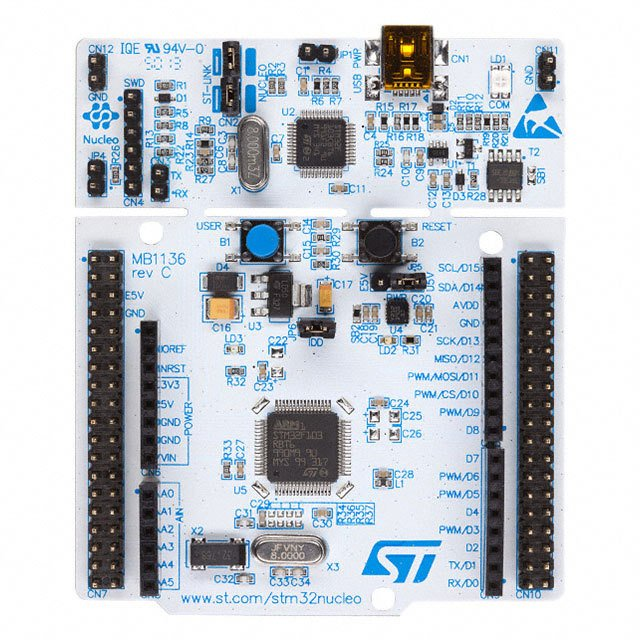
\includegraphics[width=\textwidth,height=0.3\textheight,keepaspectratio]{Figuras/nucleo.jpg}
         \caption{\centering \label{fig:a2}}
     \end{subfigure}
     ~
     \begin{subfigure}[b]{0.2\textwidth}
 	\centering
         \includegraphics[width=\textwidth,height=0.3\textheight,keepaspectratio]{Figuras/sparkfun.jpg}
         \caption{\centering \label{fig:a3}}
     \end{subfigure}
          ~
     \begin{subfigure}[b]{0.2\textwidth}
 	\centering
         \includegraphics[width=\textwidth,height=0.4\textheight,keepaspectratio]{Figuras/encoder.png}
         \caption{\centering \label{fig:a4}}
     \end{subfigure}
     
     \begin{subfigure}[b]{0.2\textwidth}
 	\centering
         \includegraphics[width=\textwidth,height=1.2\textheight,keepaspectratio]{Figuras/stepup.jpg}
         \caption{\centering \label{fig:b1}}
     \end{subfigure}
     ~
     \begin{subfigure}[b]{0.2\textwidth}
 	\centering
         \includegraphics[width=\textwidth,height=0.3\textheight,keepaspectratio]{Figuras/Lipo.png}
         \caption{\centering \label{fig:b2}}
     \end{subfigure}
     ~
     \begin{subfigure}[b]{0.2\textwidth}
 	\centering
         \includegraphics[width=0.7\textwidth,height=0.3\textheight,keepaspectratio]{Figuras/hc05.png}
         \caption{\centering \label{fig:b3}}
     \end{subfigure}
          ~
     \begin{subfigure}[b]{0.2\textwidth}
 	\centering
         \includegraphics[width=\textwidth,height=0.3\textheight,keepaspectratio]{Figuras/qre.jpg}
         \caption{\centering \label{fig:b4}}
     \end{subfigure}
     
     \caption{Materiais utilizados: (a) Motor Pololu; (b) Nucleo-STM32F303K8; (c) TB6612FNG; (d) \textit{Encoder} Pololu; (e) \textit{Step up}; (f) Bateria LiPo; (g) HC05; (h) QRE1113}     
 \end{figure}
\end{frame}

\begin{frame}
\frametitle{Softwares utilizados}

\begin{itemize}
\item Inkscape;
\item Matlab;
\item Kicad;
\item Supremica;
\item Deslab;
\item STM32 CubeMX;
\item System Workbench;
\item Linguagem C;
\item \LaTeX

\end{itemize}
\end{frame}

